\section{Methodology}

\subsection{Centralized state}
La realizzazione del sistema è stata effettuata utilizzando alcune tra le tecnologie ed i pattern più in auge nello sviluppo di applicazioni web-oriented. Nello specifico sono stati utilizzati i pattern Unidirectional Data Flow e Immutability attraverso l’implementazione messa a disposizione rispettivamente dalle librerie ReduxJS e ImmutableJS.


Lo sviluppo del progetto si è focalizzato sull'individuazione di una struttura gerarchica in grado di rappresentare in modo esaustivo l’insieme delle componenti che compongono la planimetria, costituendo di fatto lo stato dell’applicazione. Lo stato è stato gestito attraverso l’immutabilit\`a, un principio che prevede l’applicazione di nuove modifiche attraverso la generazione di un nuovo stato, in primis identico al precedente, ma sul quale vengono applicate le modifiche richieste. Dal punto di vista della gestione della memoria questo meccanismo richiederebbe un importante dispendio di risorse. Per evitare ciò l’implementazione ImmutableJS adotta dei meccanismi che simulano il principio di immutabilit\`a evitando la copia in profondit\`a della memoria  (deep clone) e alleggerendo così il carico in termini di utilizzo di memoria e tempo macchina.


\subsubsection{Application as Finite State Machine}
Per dominare la complessit\`a dell’applicazione l’intero sistema è stato modellato su una macchina a stati. Sfruttando il modello basato su azioni e reducer messo a disposizione dal pattern unidirectional data flow è stato individuato un grafo che rappresenta le possibili evoluzioni dello stato dell’applicazione. Il nodo corrente in cui si trova la macchina a stati è stato mappato attraverso l’introduzione di una variabile globale che rappresenta la modalit\`a in cui si trova l’applicazione, gli eventi del browser sono stati mappati con gli archi uscenti del grafo.Ad esempio un’operazione di creazione di un nuovo muro viene mappata attraverso un grafo composto da 4 nodi.\newline

\begin{figure}[!t]
\centering
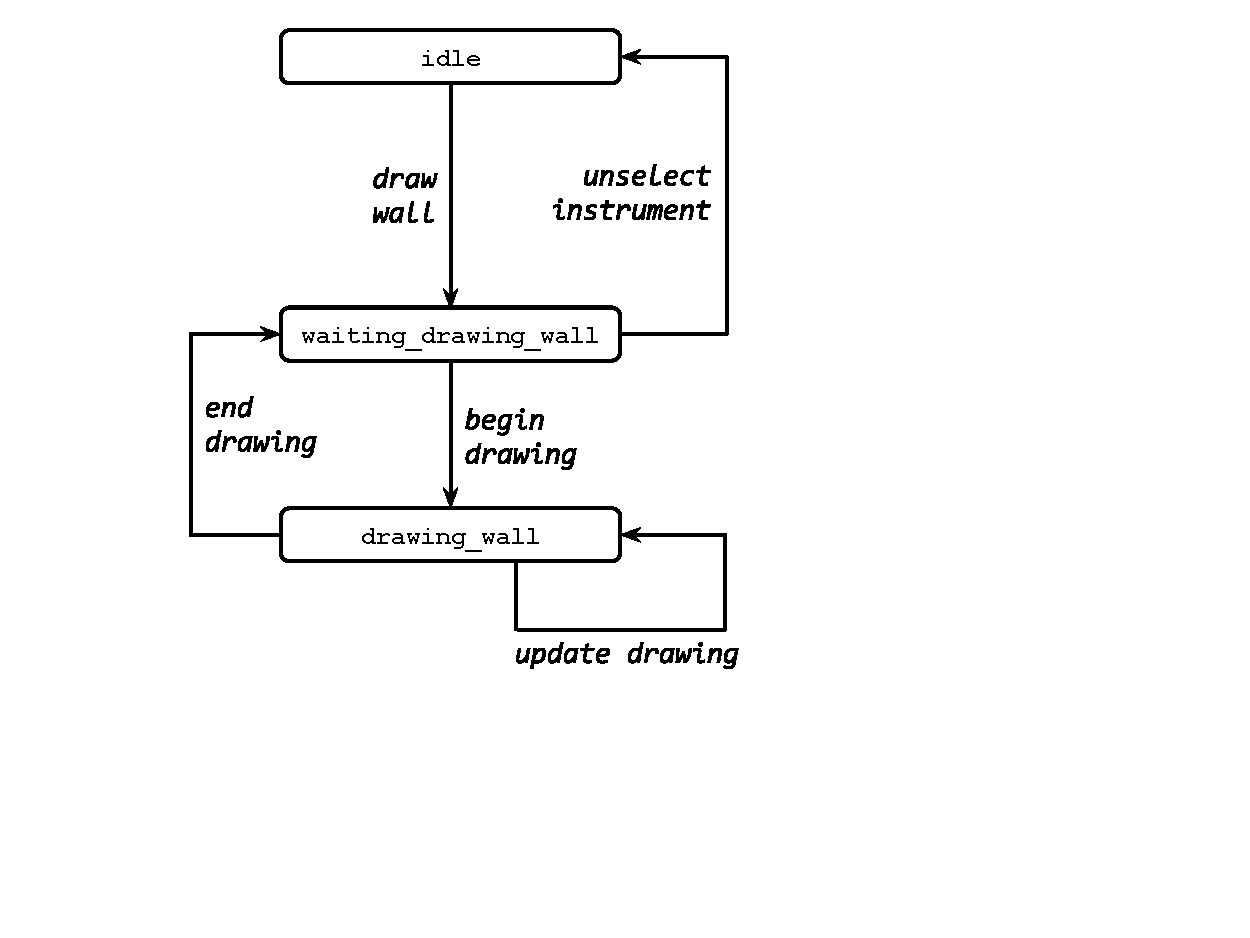
\includegraphics[width=\linewidth]{contents/images/uc_draw_wall}

\caption{Bla bla bla.}
\label{fig_sim}
\end{figure}




\subsection{Collaboration}
    COLLABORAZIONE\\

\subsection{Building elements}

L'insieme degli elementi che è possibile inserire all'interno della planimetria vengono gestiti in un catalogo, strutturato in categorie.
La categorizzazione individua un insieme di casi d'uso con cui l'utente può interagire.

\textbf{Walls}, rientrano in questa categoria tutti i tipi di muro (perimetrali, interni, portanti). La creazione avviene specificando il punto di inizio e fine dell’elemento. La rappresentazione interna viene ricondotta a quella di un grafo in cui: i \textbf{nodi} corrispondono ai punti geometrici in cui si intersecano più muri e hanno delle coordinate che li collocano nello spazio; gli \textbf{archi} corrispondono al muro.\\
\textbf{Openings}, rientrano in questa categoria gli elementi che bucano i muri come porte, finestre e archi. La creazione viene effettuata attraverso uno snap sui muri precedentemente creati. La rappresentazione interna associa ciascuna apertura con il muro di riferimento, creando un legame tra le due componenti.\\
\textbf{Areas}, rientrano in questa categoria i pavimenti. La creazione viene effettuata automaticamente attraverso un’analisi del grafo composto dai muri. L’algoritmo individuato si compone delle seguenti fasi:\\
    - Ricerca delle componenti biconnesse attraverso l'applicazione dell'algoritmo Hopcroft-Tarjan [Citazione]
    - Rimozione degli archi che non appartengono alle componenti biconnesse
    - Applicazione dell'algoritmo di ricerca del bordo per la determinazione dei cicli [Citazione]
    - Rimozione del ciclo massimale, corrispondente ad un ciclo che coinvolge tutti gli archi perimetrali del grafo attraverso la legge.... [Citazione]

\textbf{Objects}, rientrano in questa categoria tutti gli oggetti posizionabili sulle aree. L’utente può agire sulla disposizione sia in termini di posizione che rotazione.\\

\subsection{UI components}

La struttura di questa applicazione, in linea con quelli che erano gli obiettivi prefissati, permette di essere estesa cambiando i componenti che si occupano della visualizzazione dei modelli. In particolare possiamo evidenziare le seguenti parti:\\\\
\textbf{Catalogo:} contiene i plugin geometrici del sistema con tutte le loro proprietà.\\\\
\textbf{Core:} è la parte che si occupa della gestione dello stato e contiene le funzionalità di disegno prendendo le proprietà dal catalogo\\\\
\textbf{Visualizzatori:} si occupano di fornire una rappresentazione dello stato. La tipologia di visualizzatore viene scelta in base alla mode property inside state.\\\\

Uno schema dell'architettura dei visualizzatori pu\`o essere osservato nella figura~\ref{fig_visualizators}
\begin{figure}[!t]
\centering
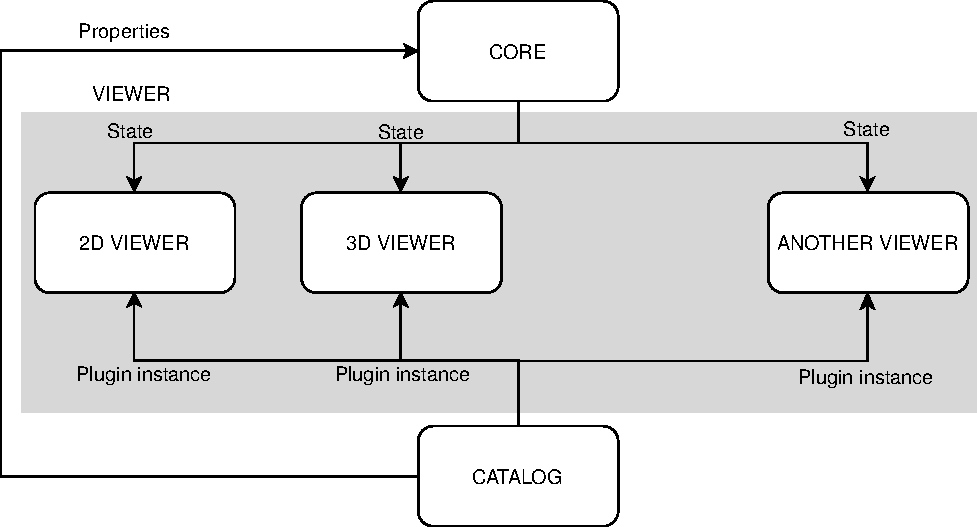
\includegraphics[width=\linewidth]{contents/images/diagramma-visualizzatori}

\caption{Bla bla bla.}
\label{fig_visualizators}
\end{figure}

\subsubsection{2D renderer component}
virtualDOM


\subsubsection{3D renderer component}
threeJS immutablediff

\subsection{Architettura serverless}
    CARICO FRONTEND\\
    CARICAMENTO REMOTO GEOMETRIA PLUGIN\\